\begin{figure}[H]
    \centering
    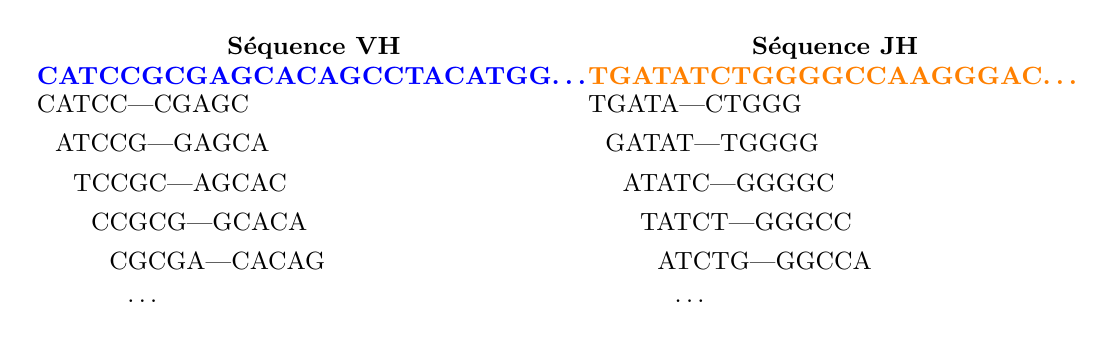
\begin{tikzpicture}[node distance=0cm, thick, font=\small]

    % Séquence VH
    \node[anchor=west] (VH) at (0,0) 
    {\shortstack{\textbf{Séquence VH} \\ \textbf{\textcolor{blue}{CATCCGCGAGCACAGCCTACATGG\dots}}}};
    
    % k-mer espacés séquence VH
    \foreach \i [count=\j from 0] in {
        CATCC---CGAGC,
        ATCCG---GAGCA,
        TCCGC---AGCAC,
        CCGCG---GCACA,
        CGCGA---CACAG,
        \dots
    } {
        \pgfmathsetmacro\xshift{\j*0.23}
        \pgfmathsetmacro\ypos{-0.5*(\j+1.1)}
        \node[anchor=west] at (\xshift,\ypos) {\i};
    }

    % Séquence JH
    \node[anchor=west] (J) at (7,0)
    {\shortstack{\textbf{Séquence JH} \\ \textbf{\textcolor{orange}{TGATATCTGGGGCCAAGGGAC\dots}}}};

    % k-mer espacés séquence JH
    \foreach \i [count=\j from 0] in {
        TGATA---CTGGG,
        GATAT---TGGGG,
        ATATC---GGGGC,
        TATCT---GGGCC,
        ATCTG---GGCCA,
        \dots
    } {
        \pgfmathsetmacro\xshift{7 + \j*0.22}
        \pgfmathsetmacro\ypos{-0.5*(\j+1.1)}
        \node[anchor=west] at (\xshift,\ypos) {\i};
    }

    \end{tikzpicture}
    \caption{
        \textit{k-mer} issus des séquences germinales \textcolor{blue}{VH (à gauche)} et 
        \textcolor{orange}{JH (à droite)} pour la génération de l'index.
    }
    \label{fig:index}
\end{figure}
